\section{Experimental validation on Grid'5000}
\label{sec:eval}

The validation of our prototype has been performed thanks to the Grid'5000
testbed \cite{grid5000}. Grid'5000 is a large-scale and versatile experimental
testbed for experiment driven research in Computer Science, which enables
researchers to get an access to a large amount of computing resources
($\sim$ 1000 nodes spread over 10 sites). This delivery of computing resources
takes the form of bare-metal machines, on which fully customised software stacks
can deployed, thus giving a very fine control of the experimental conditions.

Various tools have been developed to provide an ease of use, such as monitoring
information about networking and power consumption or programming libraries to
fine tune each aspect composing an experiment. With this in mind, we developed
our prototype using the Execo framework \cite{imbert:hal-00861886} which helped
us to deploy and configure each node composing our chosen software stack (Ubuntu
14.04, a modified version of OpenStack "devstack", and the Redis key/value store).

The validation of our work has consisted in two different scenarios. The first
scenario consisted in deploying an OpenStack infrastructure composed of 16 compute
nodes and a varying number of controllers (between 1 and 4) and to create 500 VM
creation requests, fairly distributed among the controllers, in order to detect
concurrency problems inherent in using a non relational database backend. The
second scenario consisted in creating gradually 2000 VMs on such an
infrastructure, in order to detect scalability issues whith some tasks involved
during the creation of VMs.

During this round of experiments, we compared different OpenStack
infrastructures on the basis of several criteria. To enable a fair comparison,
each infrastructure was composed of 16 compute nodes (dedicated
to the hosting of VMs) and several controllers and each infrastructure was
deployed on top of servers that delivers performance of the same order.

The default database backend that is used for storing states of OpenStack
services is MySQL, which is supposed to be deployed on a dedicated node. In the
case of this experiment, the MySQL database was hosted on one of the controller
nodes.

However using a single node dedicated to the hosting of the database exposes the
infrastructure to SPOF problems when the database node crash, a better solution
consists in using a replication mechanisms such as Galera, which enables to
distribute the MySQL database on several nodes. Its functionning is rather
simple: every database node holds the same states, and every write is performed
concurrently on every database node. Thus application can request any of the
database nodes, the data that is be return will be the same. Thanks to this
synchronization mechanism, it is possible to have distributed ACID database that
still focus on consistency and availability (CA in the CAP theorem), with the
disadvantage of an higher latency due the cost of the synchronization between
data stored on nodes.

On the other hand, Redis is a non relational database system which offer native
clustering functionning and has opted to prioritise consistency and partition
tolerance (CP in the CAP theorem). Redis thus represents an alternative to the
use of mechanisms such as MySQL+Galera.

As OpenStack services communicate with each other via RPC calls that are
intercepted by an API layer exposed by each instance of a service, we have been
able to measure the time take by each call on the API, which give a first
overview of the reactivity of a specific OpenStack configuration. Additionnaly,
measuring the time taken to spawn a given number of VMs is another way to get an
identify the reactivity of a specific configuration. 

These two metrics have been measured on several scenarios, each scenario was
involving different configurations of the following parameters:

\begin{itemize}

\item \textbf{Number of controllers}, in order to understand the impact of increasing the
number of controllers in an OpenStack deployment. This number has varied between
1 and 4.

\item \textbf{Database backend}, in order to understand the impact of using a
database backend that is different to the relational database used in Nova.

\item \textbf{Mono-site vs multi-site}, in order to measure how an OpenStack
infrastructure was performing when spread accros different geographical sites. In
such an experiment, we used 4 sites where each site was hosting 1 controller and
4 computes nodes.

\end{itemize}

\subsection{Creating 500 VMs in parallel}



\begin{table}
	\begin{tabular}[b]{|r@{\:}||@{\:}r@{\:}|@{\:}r@{\:}|@{\:}r@{\:}|}
	  \thickhline
	  \textbf{Database\ backend~~}
	    & \multicolumn{ 3 }{c@{\:}|}{Time (s) taken to create 500 VMs}
	      \Tstrut \\
	     \hfill &  ~1 CTRL~ & ~2 CTRLs~ & ~4 CTRLs~  \Bstrut \\
	  \thickhline

	     MySQL            ~~~~~~~ &  861.33~ & 497.46~ &  335.21 \\
         MySQL +Galera    ~~~~~~~ &  \multirow{1}{*}{ -- }~ & 1236.18~ &  966.41 \\
	%   Cassandra  ~~~~~~~ & 173~ & 7~ &  0 \\
	     Redis            ~~~~~~~ &  745.72~ & 533.54~ &  379.67 
	  \Rstrut  \\ \hline
	  \thickhline
	\end{tabular}
	\caption{Time spend to create 500 VMs for monosite based configurations}
	\label{tab:vm_creation_duration_monosite}
\end{table}

\begin{table}
	\begin{tabular}[b]{|r@{\:}||@{\:}r@{\:}|@{\:}r@{\:}|@{\:}r@{\:}|}
	  \thickhline
	  \textbf{Database\ backend~~}
	    & \multicolumn{ 3 }{c@{\:}|}{Time (ms) to serve API requests}
	      \Tstrut \\
	     \hfill &  ~1 CTRL~ & ~2 CTRLs~ & ~4 CTRLs~  \Bstrut \\
	  \thickhline

	     MySQL            ~~~~~~~ &  35.98~ & 40.95~ &  43.66 \\
	     MySQL +Galera    ~~~~~~~ &  \multirow{1}{*}{ -- }~ & 127.94~ &  175.67 \\
	%   Cassandra  ~~~~~~~ & 173~ & 7~ &  0 \\
	     Redis            ~~~~~~~ &  60.16~ & 79.32~ &  87.65 
	  \Rstrut  \\ \hline
	  \thickhline
	\end{tabular}
	\caption{Average time spend to serve OpenStack API requests for monosite 
	based configurations}
	\label{tab:api_duration_monosite}
\end{table}



Table~\ref{tab:api_duration_monosite} presents average of times to serve API
requests, while Table~\ref{tab:vm_creation_duration_monosite} introduces the
time taken by an OpenStack infrastructure to create 500 VMs in parallel. These
two tables presents measures that have been established for several OpenStack
configurations by varying two parameters: number of controller nodes involved in
the infrastructure and the database backend used to store OpenStack's states.


According to Table~\ref{tab:vm_creation_duration_monosite}, the time taken to
create 500 VMs in parallel decrease when the number of controller nodes involved
in the OpenStack infrastructure increase, whichever database backend is used to
store the OpenStack data states.

A deeper study with the idea of discriminating the different solutions with the
performance criterion, will state that our implementation based on the Redis
database has performance that are in the same range as those for MySQL: while
Redis is 16\% faster with one controller, with more controller nodes the gap is
closing in favor of MySQL which  becomes 13\% faster than the Redis solution.
This result is explained by the fact that in the 4 controller nodes
configuration, the Redis database will be organized in a cluster distributed and
synchronized on the 4 controller nodes, while MySQL is running only on one of
the controller nodes without any synchronization mechanism. Adding this missing
synchronization to MySQL thanks to the Galera software, has a significant impact
on the reactivity of the system: with 4 controller nodes a one node MySQL is
289\% faster that the MySQL clustered with Galera, which is in turn 255\% slower
than the Redis based solution.

On the other hand Table~\ref{tab:api_duration_monosite} shows that increasing
the number of controller nodes leads to an increase of the average time take to
process an API request. This is due to the fact that increasing the number of
controller nodes in an OpenStack configuration leads to increase of the total
workload that is required to create the 500 VMs: while the workload necessary to
spawn the VMs is distributed among the controller nodes, an extra workload arise
partially from the periodic tasks (network, storage, ...) that are run by
controller nodes to heal the infrastructure, the remaining extra workload coming
from mechanisms to prevent concurrency issues and race condition when
manipulating OpenStack states. Furthermore, the addition of controller nodes
leads to an increase of the probability that several controller nodes manipulate
a same resource stored in OpenStack's states, thus requiring mechanisms to
organize race conditions. In such a situation, a single MySQL node looks better
with an average of 43.66 ms to serve API requests in a 4 controller nodes
configuration. Clustered database deployments require a significantly higher
time to server API requests: in the same 4 controller nodes configuration, Redis
is 101\% slower than the non clustered MySQL, while the clustered MySQL with
Galera is 302\% slower than then non clustered one.

In this first set of experiments, a single node MySQL is the more performant
solution as it is faster the faster solution in term of time to spawn 500 VMs
and in term of time to serve API requests, but at the cost of a lack of
synchronization mechanisms which make this solution unrelevant for fault
tolerance reasons. If the fault tolerant solutions are considered, using a
clustered KVS become a bette choice as it doesn't penalize OpenStack
functionning and offers better performances than the Galera cluster and provide
a fault tolerant functionning.

% According to Table~\ref{tab:api_duration_monosite}, increasing the number of
% controllers in the deployment leads to an increase of the average time spend to
% serve API requests. This results is explained by the fact that controllers do
% most of the work during the creation of VM, and increasing the number of
% controllers enables to distribute this workload on several entities that works
% in parallel. This last point is confirmed by
% Table~\ref{tab:vm_creation_duration_monosite}, where it is clear that increasing
% the number of controllers in the deployment accelerate the processus of creating
% the VMs.

% Regarding the database systems, even if using a single MySQL node leads to SPOF
% problems, as it doesn't take into account fault tolerance in its functionning,
% it is normal that it delivers the best performance, which can be considered as a
% standard of performance that can be fairly used to position performances of
% alternative systems that take into account fault tolerance. According to this,
% results extracted from Table~\ref{tab:api_duration_monosite} are easily
% explained as Redis and Galera implement synchronisation/fault tolerance
% mechanisms while serving requests for data. Indeed with Redis, the average time
% to serve API request is twice the time measured with MySQL, and is about 3 time
% lower than the time measured with Galera based requests. It is noticeable that




\subsection{Creating 2000 VMs gradually}

%  that through 10 different Nova controllers deployed on one cluster located
% in Nantes. This experiment enabled us to confirm that OpenStack's
% services were working correctly with the key/value store.
% that the relational backend
%used by the several components can be satisfactorily replaced by this
%new distributed key/value system.
% Although further experiments are
% required to test the scalability as well as the effect
% of geographical distances on the reliability and efficiency, we are
% confident about our approach as several distributed key/value stores
% are already used WANWide.

% \AL[JP]{Finalize the text of this section, please be consistent the
%   announcement at the end of the introduction}
% Several test-cases with 10 nodes to evaluate
% the efficiency of the new framework:\begin{inparaenum}[1\upshape)]
% \item 1 site, 1 controller, 9 compute nodes
% \item 1 site, 10 controllesr, 0 compute node
% \item 2 sites, 1 controller/by site, 4 compute nodes/by site
% \item and 2 sites, 5 controllers/by site, 0 compute nodes/by site
% \end{inparaenum}



%test infrastructure is a tedious task if one has to do it
%manually. In order to simplify tests, we create a tool based on \texttt{Execo}
%\cite{imbert:hal-00861886} that: find a time slot when the resources
%are available on the several sites.
% deploy Ubuntu 14.04 on all the nodes, install RIAK DB and setup
% our modified version of devstack (with automatic node configuration), and
% finally start the distributed OpenStack infrastructure. The duration of the
% deployment is around 1 hour, depending on the cluster hardware and the
% total number of nodes. Finally, the tool provides some options that simplifies
% the management of the different test-cases, namely the number of sites,
% controller by site and compute nodes by site.

%\begin{figure}[h!]
%    \centering
%    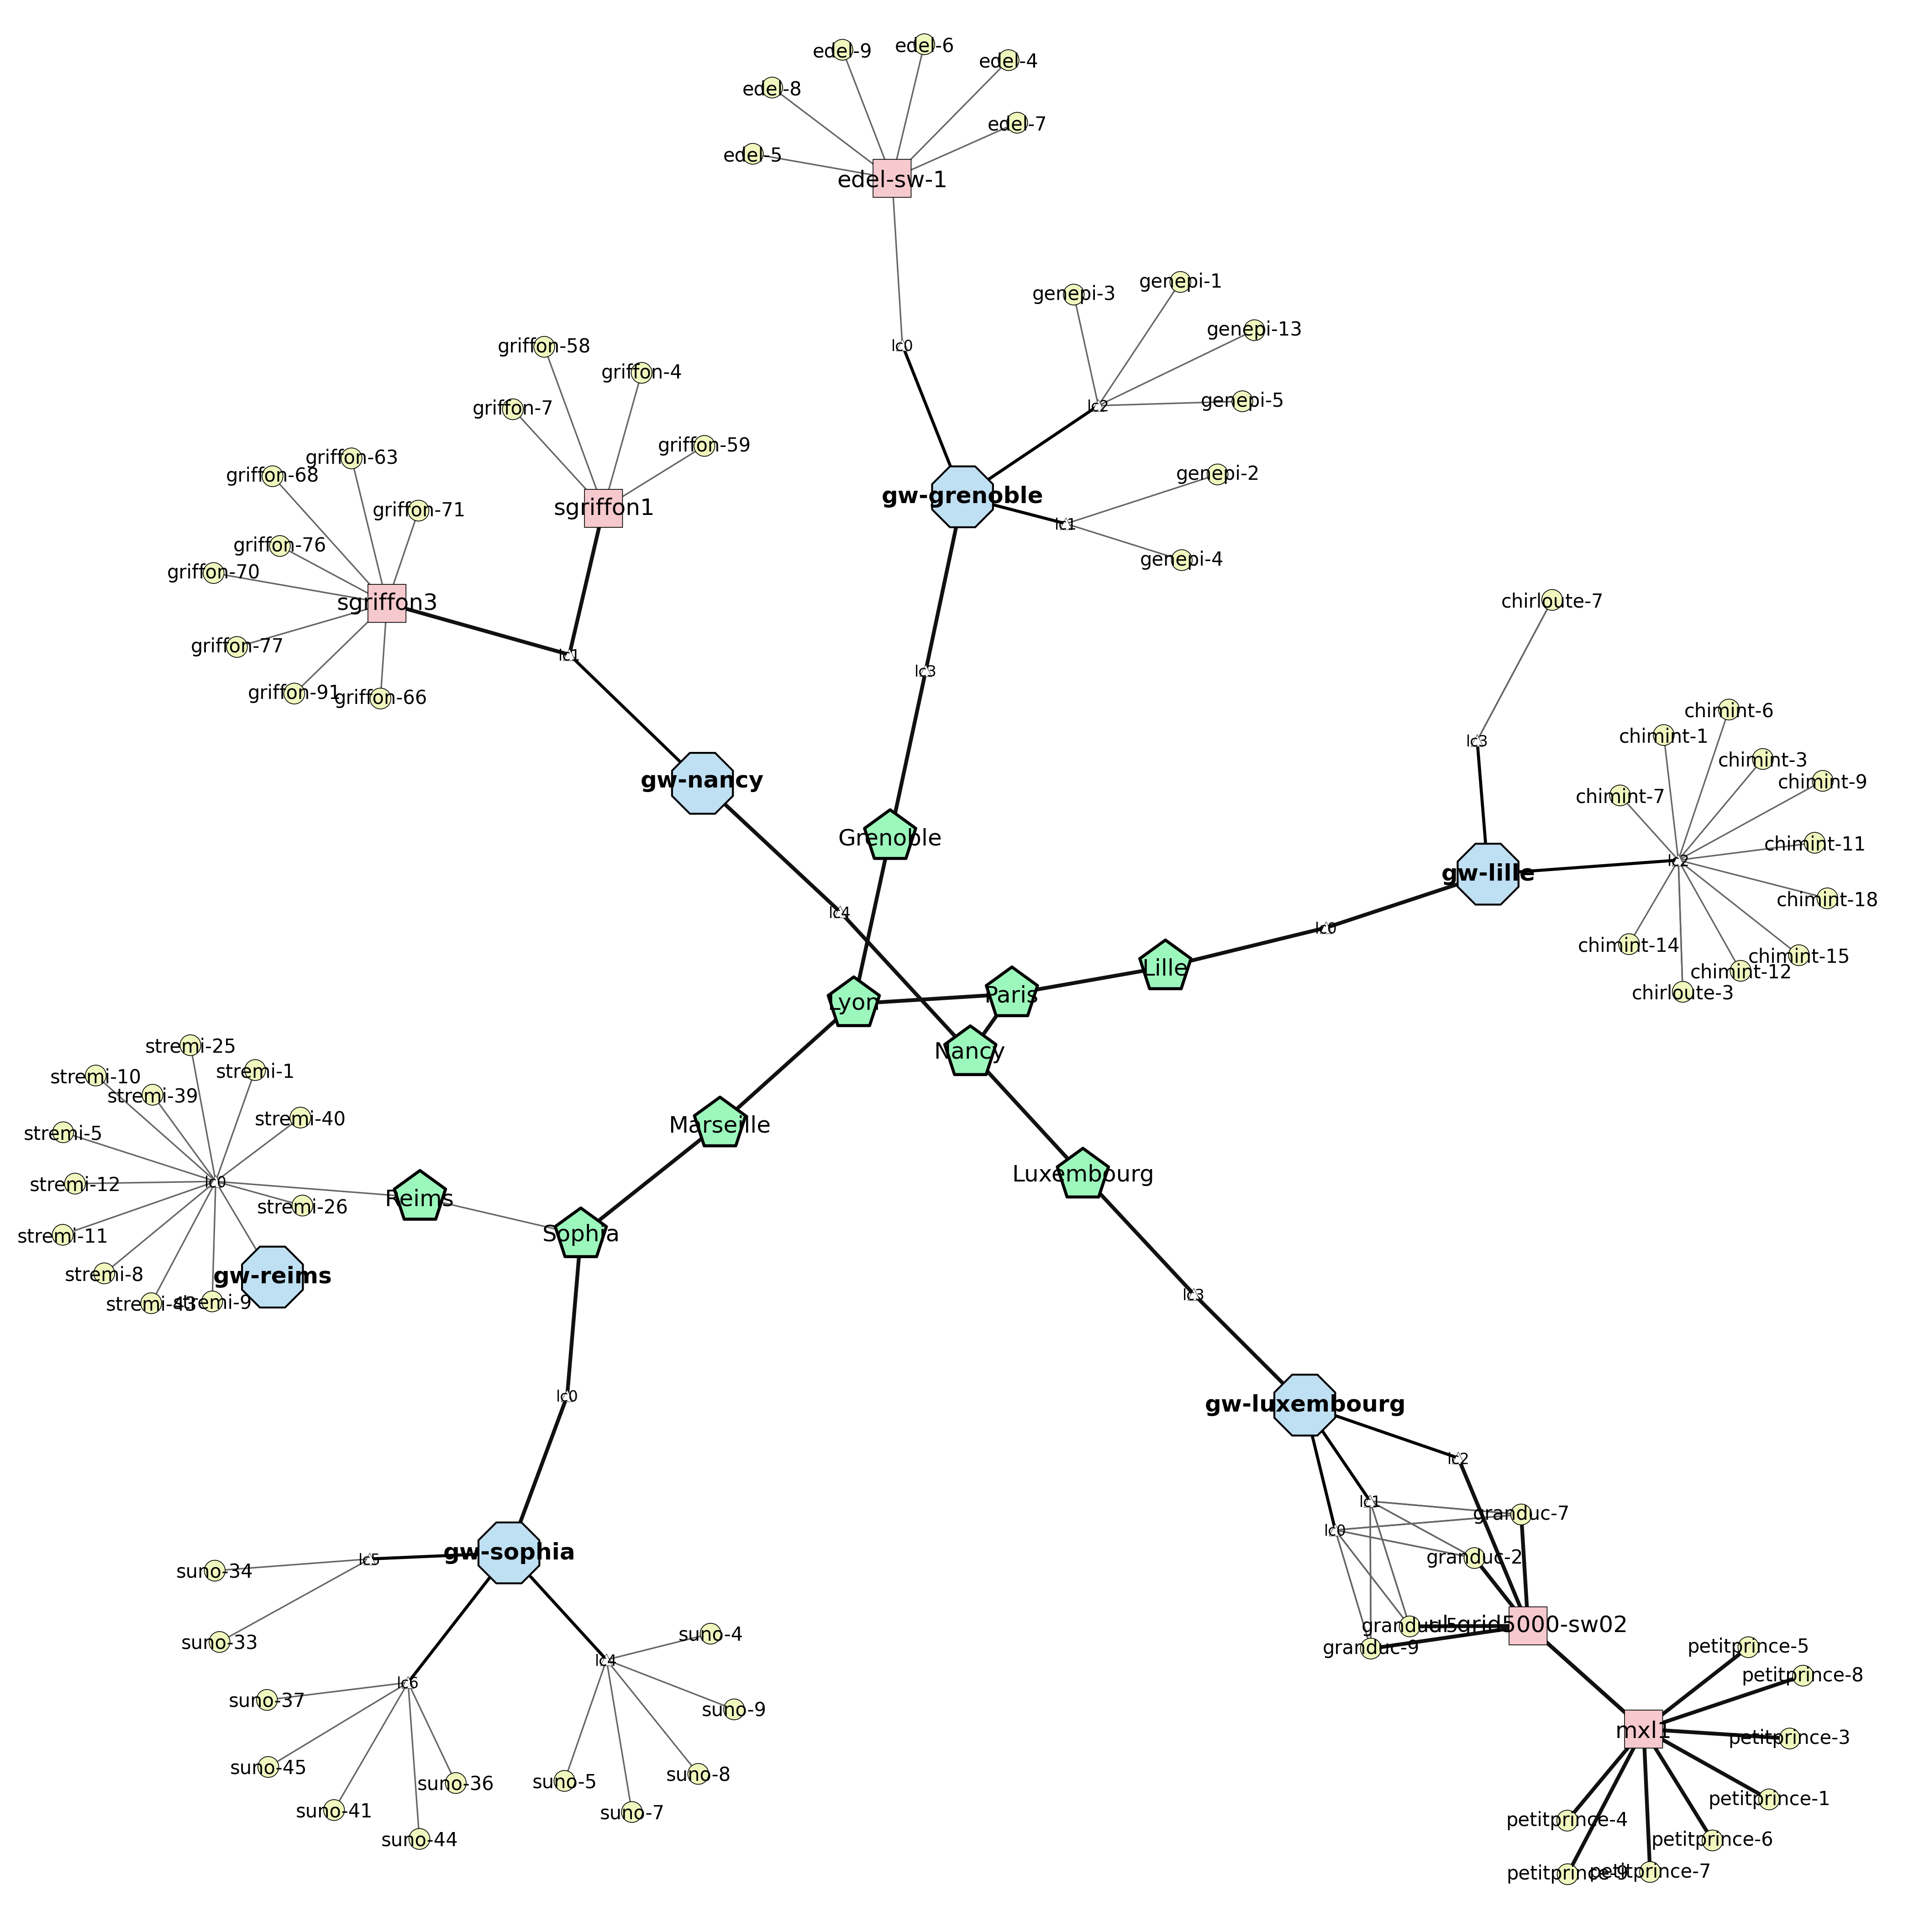
\includegraphics[width=7cm]{figures/6_sites.png}
%    \caption{Test-cases on the Grid'5000 platform involving 6
%    geographically-spreaded sites each hosting 2 controllers and 10 computes
%    nodes.}
%\end{figure}


%\subsubsection{Test-cases}
%\paragraph{Monosite}
%\paragraph{Multisite: 1 controller per site}
%\paragraph{Multisite: 10 controllers per site}
